\begin{figure}[t!]
\centering
  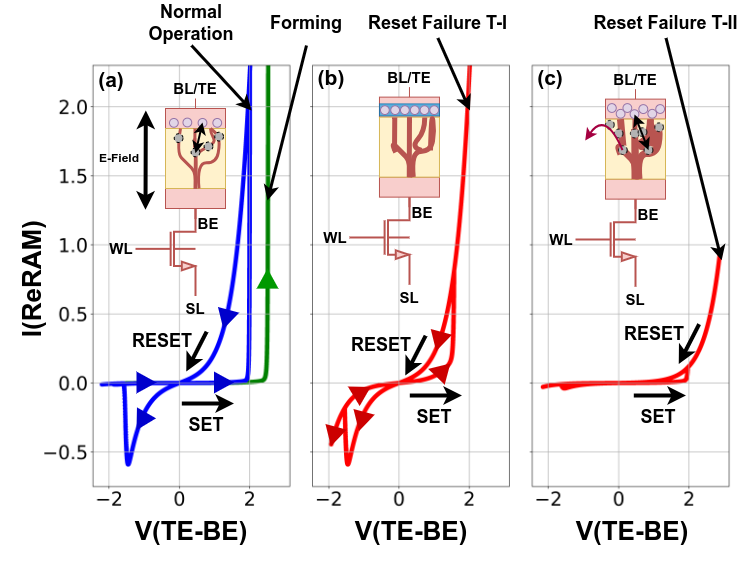
\includegraphics[width=0.9\linewidth]{img/hysteresis_annot.png}
  \caption{Hysteresis curves for a Skywater 130nm ReRAM 1T1R macro. The ReRAM cell is modeled using the Stanford-PKU macro Verilog-A model. Default parameters are assumed. Various stages of aging are modeled by limiting the filament minimum and maximum area parameter to provide a coarse-grained example of ReRAM wear-out. Subplot \textbf{(a)} depicts the hysteresis curve of a fresh cell. Subplot \textbf{(b)} is the result of increasing the minimum filament size, which may lead to \cite{chen2011reram} an error whose characteristic is a convergence of SET/RESET resistance leading to a decrease in the resistance ratio. This effect is believed to be caused by electrode oxidization. Subplot \textbf{(c)} is the result of limiting both SET and RESET filament sizes. This effect is believed to be caused by extra vacancies appearing due to electric field exposure enlarging the filament leading to the failure of the RESET operation and a resistance ratio to decrease \cite{chen2011reram}.}
\label{fig:hyst_reram}
\end{figure} 